\subsection{Building a mesh}

\begin{frame}
    \frametitle{Examples}

    \begin{figure}[!ht]
        \centering
        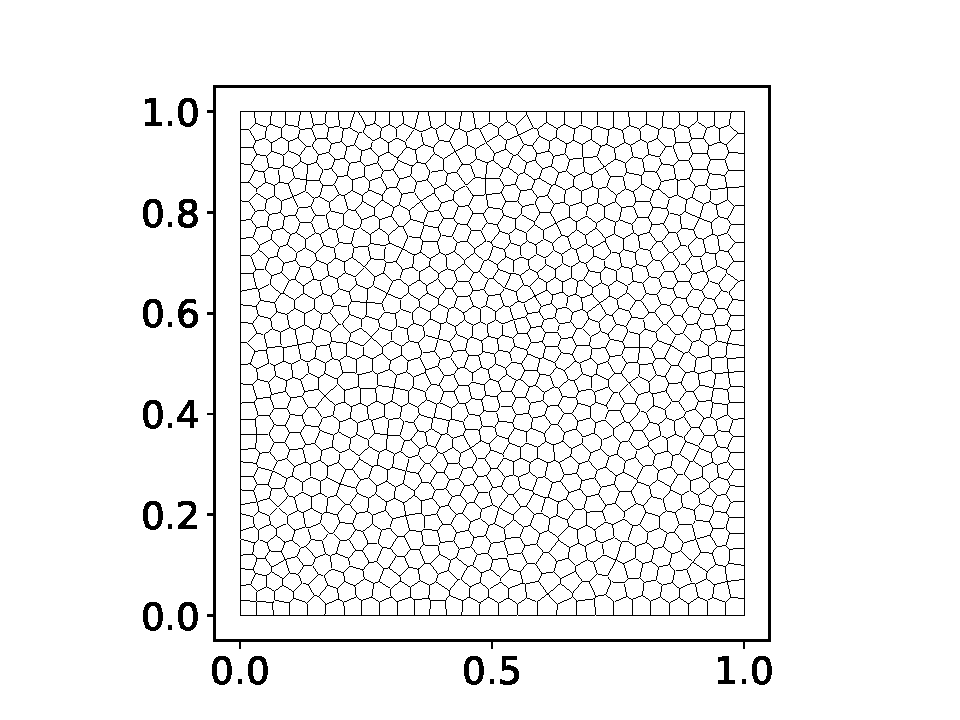
\includegraphics[trim=2cm 0.5cm 2cm 0.5cm, clip, width=0.45\textwidth]{meshes/uniform/square_1000.pdf}
        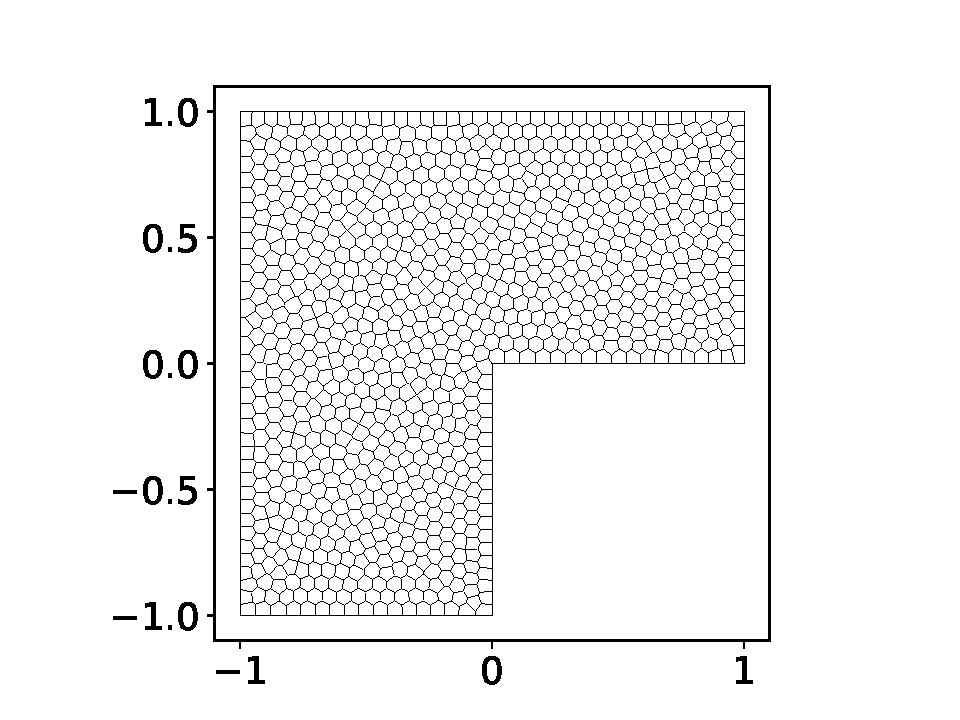
\includegraphics[trim=2cm 0.5cm 2cm 0.5cm, clip, width=0.45\textwidth]{meshes/uniform/lshape_1000.pdf}
        \caption{Square and L-shaped meshes over polygonal domains with $N = 1000$ elements.}
    \end{figure}
\end{frame}

\begin{frame}
    \frametitle{Mesh-Building Strategy}

    The mesh-building strategy follows these steps:

    \begin{enumerate}
        \item Voronoi diagram generation,
        \item Diagram relaxation,
        \item Small edge collapse,
        \item Element connectivity analysis,
        \item Property evaluation.
    \end{enumerate}

    This process is facilitated by a thorough implementation of analytic geometry operations, including those involving lines and polygons.
\end{frame}

\begin{frame}[fragile]
    \frametitle{\lstinline{mesh_diagram}, \lstinline{mesh_relax}}

    Most steps of the mesh-building process are carried out by \lstinline{mesh_diagram}\footnote{Building and postprocessing.} and \lstinline{mesh_relax}.

    \begin{lstlisting}[style=cpp]
    std::vector<Polygon> mesh_diagram(
        const Polygon &, 
        const std::size_t &, 
        const bool &reflect = false, 
        const bool &uniform = false);

    std::vector<Polygon> mesh_relax(
        const Polygon &, 
        const std::vector<Polygon> &, 
        const bool &reflect = false);
    \end{lstlisting}

\end{frame}

\begin{frame}[fragile]
    \frametitle{\lstinline{Mesh}}

    \lstinline{struct Mesh} requires a polygonal domain, a diagram, and information on the elements' degrees.

    \begin{lstlisting}[style=cpp]
    Mesh(
        const Polygon &, 
        const std::vector<Polygon> &, 
        const std::vector<std::size_t> &);

    Mesh(
        const Polygon &, 
        const std::vector<Polygon> &, 
        const std::size_t &degree = 1);
    \end{lstlisting}

\end{frame}

\begin{frame}[fragile]
    \frametitle{\lstinline{Mesh} methods}

    The following methods are invoked by the mesh constructors to evaluate the diagram's properties.

    \begin{lstlisting}[style=cpp]
    std::vector<Element> mesh_elements(
        const std::vector<Polygon> &, 
        const std::vector<std::size_t> &);

    std::vector<std::vector<std::array<int, 3>>> 
    mesh_neighbours(
        const Polygon &, 
        const std::vector<Element> &);

    std::vector<Real> mesh_areas(
        const std::vector<Polygon> &);

    std::vector<Vector<Real>> mesh_max_simplices(
        const std::vector<Polygon> &);
    \end{lstlisting}

\end{frame}

\subsection{Code examples}

\begin{frame}[fragile]
    \frametitle{A code snippet}

    The steps to create a mesh are schematized as follows:

    \begin{lstlisting}[style=cpp]
    Point a{0.0, 0.0};
    Point b{1.0, 0.0};
    Point c{1.0, 1.0};
    Point d{0.0, 1.0};

    Polygon domain{{a, b, c, d}};

    std::vector<Polygon> diagram = 
        mesh_diagram(domain, 100);
    
    Mesh mesh{domain, diagram};
    \end{lstlisting}

\end{frame}

\begin{frame}[fragile]
    \frametitle{A repository snippet}

    Building a mesh over a square or L-shaped domain is as simple as calling one of the two scripts provided with the repository.

    To create a mesh over a square domain with $N = 250$, simply compile the domain scripts by:

    \begin{lstlisting}
    make domains
    \end{lstlisting}

    and then use the \lstinline{square_domain} script by:

    \begin{lstlisting}
    ./executables/square_domain.out 250
    \end{lstlisting}

\end{frame}